
\documentclass{beamer}
\usepackage{HECbeamer}
\usepackage{icomma}
\usepackage{numprint}
\title[\color{white}{MATH 60604 \S~6b - Données corrélées}]{\texorpdfstring{MATH 60604 \\Modélisation statistique \\ \S~6b - Données corrélées}{MATH 60604 \\Modélisation statistique \\ \S~6b - Données corrélées}}
\author{}
\institute{HEC Montréal\\
Département de sciences de la décision}
\date{}

\begin{document}
\frame{\titlepage}

%

\begin{frame}[fragile]
\frametitle{Exemple: mobilisation au travail}
 On considère des données corrélées par groupe.

\bi
\item  Une grande entreprise a procédé à une collecte de données auprès de ses
employés à l'aide d'un questionnaire.
\item La variable réponse est la \alert{mobilisation au travail}.
\item L'échelle de mobilisation au travail est
définie comme étant la somme de trois items du questionnaire, à savoir
\bi
\vp
\item Je partage plusieurs des valeurs de l'entreprise.
\item Je me sens loyal à l'entreprise.
\item Je suis fier de dire aux gens pour quelle entreprise je travaille.
\ei
mesurés sur une échelle de
Likert à cinq points allant de fortement en désaccord (\texttt{1}) à fortement en accord (\texttt{5}).
\item Les données sont inspirées de l'étude
\begin{quote}
Lee, H.-J. et Peccei, R. (2007). \textsl{Organizational-Level Gender Dissimilarity and
Employee Commitment}. British Journal of Industrial Relations, \textbf{45}, 687--712.
\end{quote}
\ei
\end{frame}

\begin{frame}[fragile]
\frametitle{Données \texttt{mobilisation}}
\bi
\item  Les données \code{mobilisation.sas7bdat} contiennent les variables
\bi
\vp
\item \code{nunite}: nombre d'employé dans l'unité (département).
\item \code{idunite}: identification de l'unité (département) où travaille l'employé.
\item  \code{idemploye}: identifiant de l'employé à l'intérieur de l'unité.
\item \code{anciennete}: ancienneté de l'employé (en années).
\item \code{sexe}: sexe de l'employé, soit homme (\texttt{0}) ou femme (\texttt{1}).
\item  \code{agegest}: âge du gestionnaire de l'unité (en années).
\item \code{mobilisation}: score à l'échelle de mobilisation.
\ei
\item Une \alert{source possible de corrélation} entre les observations est \alert{l'unité d'appartenance}.
\item Il est en effet probable que la mobilisation soit affectée par l'unité d'appartenance à cause de facteurs tels le climat de travail, le type de travail effectué par les employés et ainsi de suite.
\ei
\end{frame}


\begin{frame}[fragile]
\frametitle{Statistique descriptive}
Dans les données \texttt{mobilisation}, le nombre d'employé par unité varie.
Par exemple, l'unité $1$ a neuf employés (trois femmes et six hommes).
\begin{center}
 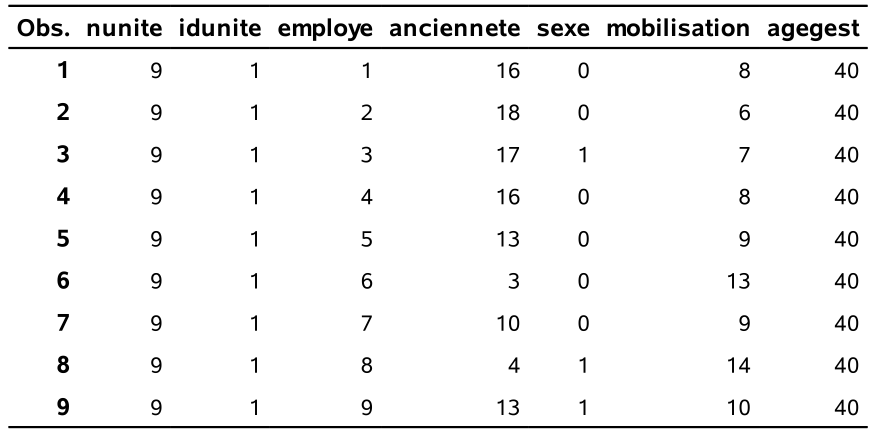
\includegraphics[width = 0.7\linewidth]{img/c6/diapos7-e06}
\end{center}
{\small
% \item The years of service of the employees for this unit varies from three to $18$.
% \item The manager for this unit is $40$ years old.
Il y a deux types de variables qui peuvent être incluses dans le modèle:
\be

\item celles quis sont fixes pour tous les individus de l'unité (\code{nunite} et \code{agegest})
\item celles qui changent selon les individus (\code{anciennete} et \code{sexe}).
\ee
}
\end{frame}


\begin{frame}[fragile]
\frametitle{Variable de regroupement et objectifs de l'étude}
\bi
\item Dans le cas des données \texttt{vengeance}, le groupe était l'individu et on a considéré seulement des variables explicatives fixes dans le temps, à part bien sûr la variable temps elle-même.
\item Ici, il y a $100$ unités en tout et $1016$ observations dans le fichier.
\item Le but de l'étude est d'évaluer l'impact du sexe, de l'ancienneté, de la taille de l'unité et de l'âge du gestionnaire sur la mobilisation.
\item Il faut tenir compte de la possible corrélation intra-unité. Il n'y a pas d'ordre naturel pour les observations au sein d'une unité (contrairement aux données \texttt{vengeance} qui contenait des données répétées dans le temps).
\ei
\end{frame}
\begin{frame}[fragile]
\frametitle{Structure de covariance pour la mobilisation}
\bi
\item On considère le modèle d'équicorrélation intra-unité pour la corrélation.
\bi

\item Cela signifie que la corrélation (conditionnelle) pour chaque paire d'observations (d'employés) est la même au sein de l'unité.
\ei
   \ei
 \begin{tcolorbox}[colback=white, colframe=hecblue, title=Code \SASlang pour le modèle linéaire avec erreurs équicorrélées]
 \begin{small}
\begin{verbatim}
proc mixed data=modstat.mobilisation method=reml;
class idunite;
model mobilisation = sexe anciennete agegest
        nunite / solution;
repeated / subject=idunite type=cs r=1 rcorr=1;
run;
\end{verbatim}
\end{small}
\end{tcolorbox}

\end{frame}


 \begin{frame}
\frametitle{Matrice de covariance intra-unité (unité 1)}
\begin{center}
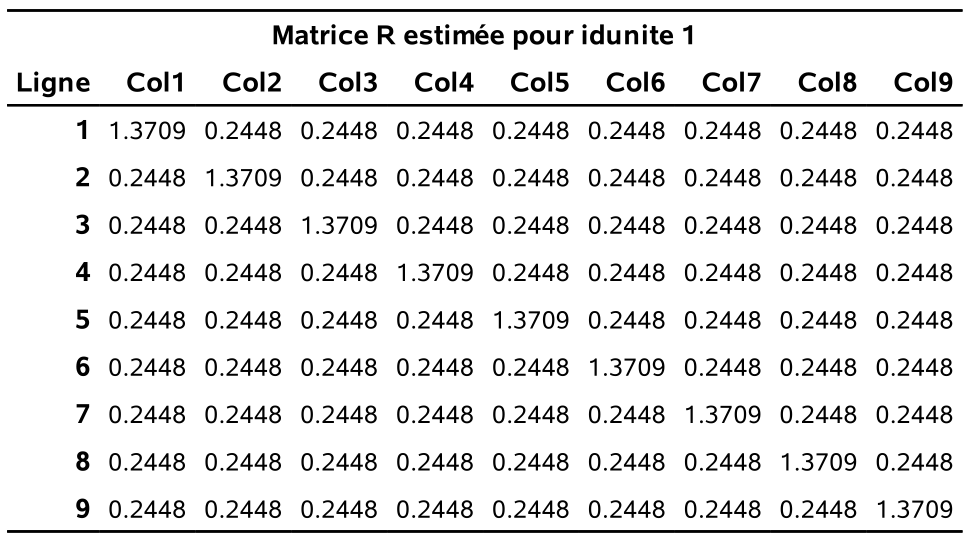
\includegraphics[width = 0.85\linewidth]{img/c6/diapos7-e07}

\end{center}
\end{frame}

 \begin{frame}
\frametitle{Modèle d'équicorrélation intra-unité}
\begin{center}
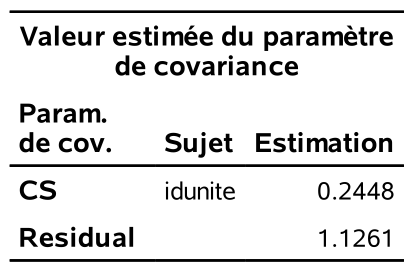
\includegraphics[width = 0.42\linewidth]{img/c6/diapos7-e08}
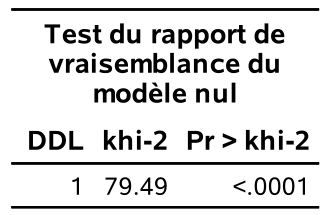
\includegraphics[width = 0.32\linewidth]{img/c6/diapos7-e09}
\end{center}
\bi
\item L'estimé du paramètre de covariance du modèle d'équicorrélation est $\hat{\tau} = 0,2448$ et il est significativement différent de zéro. Cela suggère une association positive entre la mobilisation des travailleurs au sein de l'unité, après avoir pris en compte l'effet des variables explicatives.
\item L'estimé de la corrélation entre deux travailleurs intra-unité  est $\hat{\rho} = 0,1785$.
\ei
\end{frame}



 \begin{frame}
\frametitle{Estimés des effets fixes}
\begin{center}
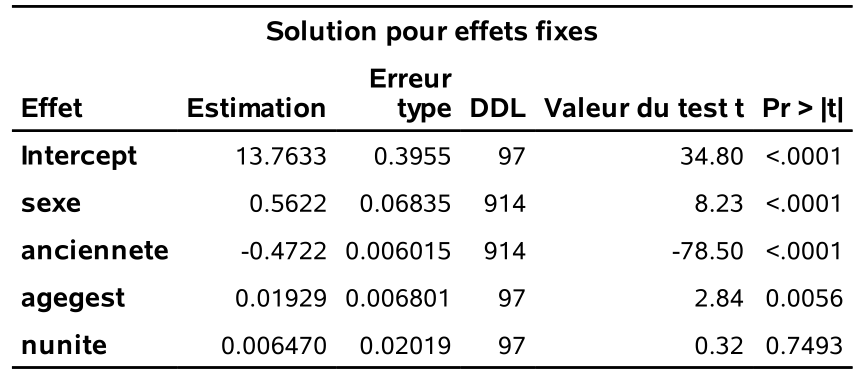
\includegraphics[width = 0.7\linewidth]{img/c6/diapos7-e10}
\end{center}
\bi
\item Trois des variables explicatives sont significatives : \code{sexe}, \code{anciennete} et \code{agegest}:
\bi
\item Les femmes sont plus mobilisées que les hommes en moyenne.
\item Plus l'employé a de l'ancienneté, moins il est mobilisé.
\item Plus le gestionnaire est âgé, plus l'employé est mobilisé.
\ei
\item Par contre, la taille de l'unité  n'est pas significative, au-delà des autres variables.
\ei
\end{frame}

\begin{frame}[fragile]
\frametitle{Exemple: mobilisation au travail}
\bi
\item Il pourrait être intéressant d'incorporer un effet unité dans le modèle.
\item En ajoutant un effet fixe au niveau du groupe, on perd en revanche la possibilité d'estimer les effets des variables qui sont fixes au niveau du groupe.
\item Ça voudrait dire qu'on ne pourrait pas inclure les variables \code{agegest} et \code{nunite}.
\item Il existe une façon de quand même incorporer un effet groupe, tout en conservant la possibilité d'avoir des variables fixes au niveau du groupe.
\item Il s'agit d'utiliser des \alert{effets aléatoires} plutôt que des effets fixes.
\item De plus, nous verrons que les effets aléatoires servent aussi à modéliser la structure de covariance.
\ei
\end{frame}
\end{document}
